\chapter[Paleoclima e nicho climático passado]{Paleoclima, Nicho Climático Passado e Reconstrução Histórica da Distribuição}

\begin{objetivos}
	Ao final desta unidade, o estudante deverá compreender como dados paleoclimáticos podem ser usados em SDM; reconhecer períodos como Holoceno Médio, Último Máximo Glacial e Último Interglacial; preparar camadas paleoclimáticas compatíveis com os modelos atuais; projetar modelos de \textit{Dinizia excelsa} para climas passados; avaliar estabilidade climática histórica; identificar possíveis áreas de refúgio; e interpretar o nicho climático passado como componente da história biogeográfica da espécie.
\end{objetivos}

\section{Introdução}

A distribuição atual de uma espécie arbórea amazônica é resultado de processos ecológicos contemporâneos e de uma história climática profunda. Mudanças passadas em temperatura, precipitação, sazonalidade, conectividade florestal e estabilidade ambiental podem ter influenciado a persistência, expansão, retração e estruturação espacial das populações.

Em Modelagem de Distribuição de Espécies, reconstruções paleoclimáticas permitem projetar modelos calibrados no presente para períodos passados, como o Holoceno Médio, o Último Máximo Glacial e o Último Interglacial. Essas projeções ajudam a formular hipóteses sobre estabilidade climática, refúgios, conectividade histórica e conservação de nicho.

\begin{conceito}[title={\faBook\quad Nicho climático passado}]
	O nicho climático passado representa o conjunto de condições ambientais históricas que poderiam ter favorecido a persistência, expansão ou retração de uma espécie ao longo do tempo geológico recente.
\end{conceito}

%------------------------------------------------
\section{Linha do tempo paleoclimática e cenários futuros}
%------------------------------------------------

A modelagem paleoclimática permite reconstruir a distribuição potencial das
espécies sob condições ambientais do passado, enquanto as projeções futuras
permitem avaliar possíveis respostas sob cenários de mudanças climáticas. Em
conjunto, essas abordagens conectam biogeografia histórica, estabilidade
climática, refúgios ecológicos e vulnerabilidade futura.

Nesta unidade, o nicho climático de \textit{Dinizia excelsa} é interpretado ao
longo de uma linha temporal que integra períodos paleoclimáticos clássicos,
condições climáticas atuais e cenários futuros derivados de modelos climáticos
globais. Essa perspectiva temporal amplia a interpretação dos modelos, pois
permite investigar se áreas atualmente adequadas também foram estáveis no
passado e se tendem a permanecer adequadas sob mudanças climáticas futuras.

\begin{center}
	\fbox{
		\begin{minipage}{0.88\textwidth}
			
			\centering
			\textbf{Linha do tempo climática utilizada na interpretação dos modelos}
			
			\vspace{0.4cm}
			
			\begin{tabular}{c c p{0.48\textwidth}}
				\toprule
				\textbf{Tempo} & \textbf{Período/Cenário} & \textbf{Interpretação ecológica} \\
				\midrule
				
				130 ka &
				Último Interglacial (LIG) &
				Período quente anterior ao último ciclo glacial, útil para avaliar respostas da espécie a condições mais quentes que as atuais. \\
				
				21 ka &
				Último Máximo Glacial (LGM) &
				Fase fria e seca do último ciclo glacial, associada a mudanças expressivas na distribuição de ambientes tropicais. \\
				
				6 ka &
				Holoceno Médio &
				Período pós-glacial com reorganização climática e ecológica, importante para inferir estabilidade recente de áreas adequadas. \\
				
				0 ka &
				Presente &
				Condição climática de referência usada para calibrar ou interpretar os modelos atuais. \\
				
				2050 &
				SSP126 &
				Cenário futuro de menor emissão, usado para avaliar respostas sob mitigação climática. \\
				
				2050 &
				SSP585 &
				Cenário futuro de alta emissão, representando maior pressão climática sobre a distribuição potencial. \\
				
				2070 &
				SSP126 &
				Projeção de médio-longo prazo sob cenário de menor emissão. \\
				
				2070 &
				SSP585 &
				Projeção de médio-longo prazo sob cenário de alta emissão e maior risco de perda de adequabilidade. \\
				
				\bottomrule
			\end{tabular}
			
		\end{minipage}
	}
\end{center}

Essa linha do tempo deve ser interpretada como uma estrutura conceitual para
comparar estabilidade, perda, ganho e deslocamento de áreas climaticamente
adequadas ao longo de diferentes janelas temporais. Áreas que permanecem
adequadas desde o passado até o futuro podem indicar maior estabilidade
climática e potencial importância como refúgios biogeográficos. Por outro lado,
áreas adequadas apenas no presente ou apenas em cenários futuros devem ser
interpretadas com cautela, especialmente quando associadas à extrapolação
ambiental.

\begin{center}
	\fbox{
		\begin{minipage}{0.90\textwidth}
			
			\textbf{Mensagem-chave.}
			
			A integração entre paleoclima, clima presente e cenários futuros transforma a
			SDM em uma ferramenta temporal. O objetivo deixa de ser apenas mapear onde a
			espécie pode ocorrer hoje e passa a incluir perguntas sobre estabilidade
			histórica, persistência climática, vulnerabilidade futura e identificação de
			possíveis refúgios para conservação.
			
		\end{minipage}
	}
\end{center}

\section{Períodos paleoclimáticos relevantes}

Nesta unidade, trabalharemos com três janelas temporais principais:

\begin{itemize}
	\item Holoceno Médio, aproximadamente 6 mil anos antes do presente;
	\item Último Máximo Glacial, aproximadamente 21 mil anos antes do presente;
	\item Último Interglacial, aproximadamente 120 mil anos antes do presente.
\end{itemize}

Esses períodos representam diferentes estados climáticos do sistema terrestre e permitem avaliar se áreas atualmente adequadas para \textit{Dinizia excelsa} também apresentavam adequabilidade no passado.

\begin{atencao}[title={\faExclamationTriangle\quad Projeções paleoclimáticas são hipóteses}]
	Mapas paleoclimáticos em SDM não demonstram ocorrência passada da espécie. Eles indicam áreas que poderiam ter sido climaticamente adequadas, assumindo conservação parcial do nicho e compatibilidade entre clima passado e modelo atual.
\end{atencao}

\section{Preparação das camadas paleoclimáticas}

As camadas paleoclimáticas devem ser harmonizadas com as variáveis atuais utilizadas no ajuste dos modelos. Isso inclui nomes, resolução, extensão, projeção e máscara espacial.

\rscriptfile{scripts/unidade15/01_estrutura_pastas.R}

\rscriptfile{scripts/unidade15/02_preparar_variaveis_paleoclimaticas.R}

\section{Projeção dos modelos para o passado}

Os modelos ajustados no presente são projetados para os cenários paleoclimáticos. Essa etapa permite comparar a adequabilidade atual com adequabilidade sob climas passados.

\rscriptfile{scripts/unidade15/03_projetar_modelos_passado.R}

\begin{figure}[H]
	\centering
	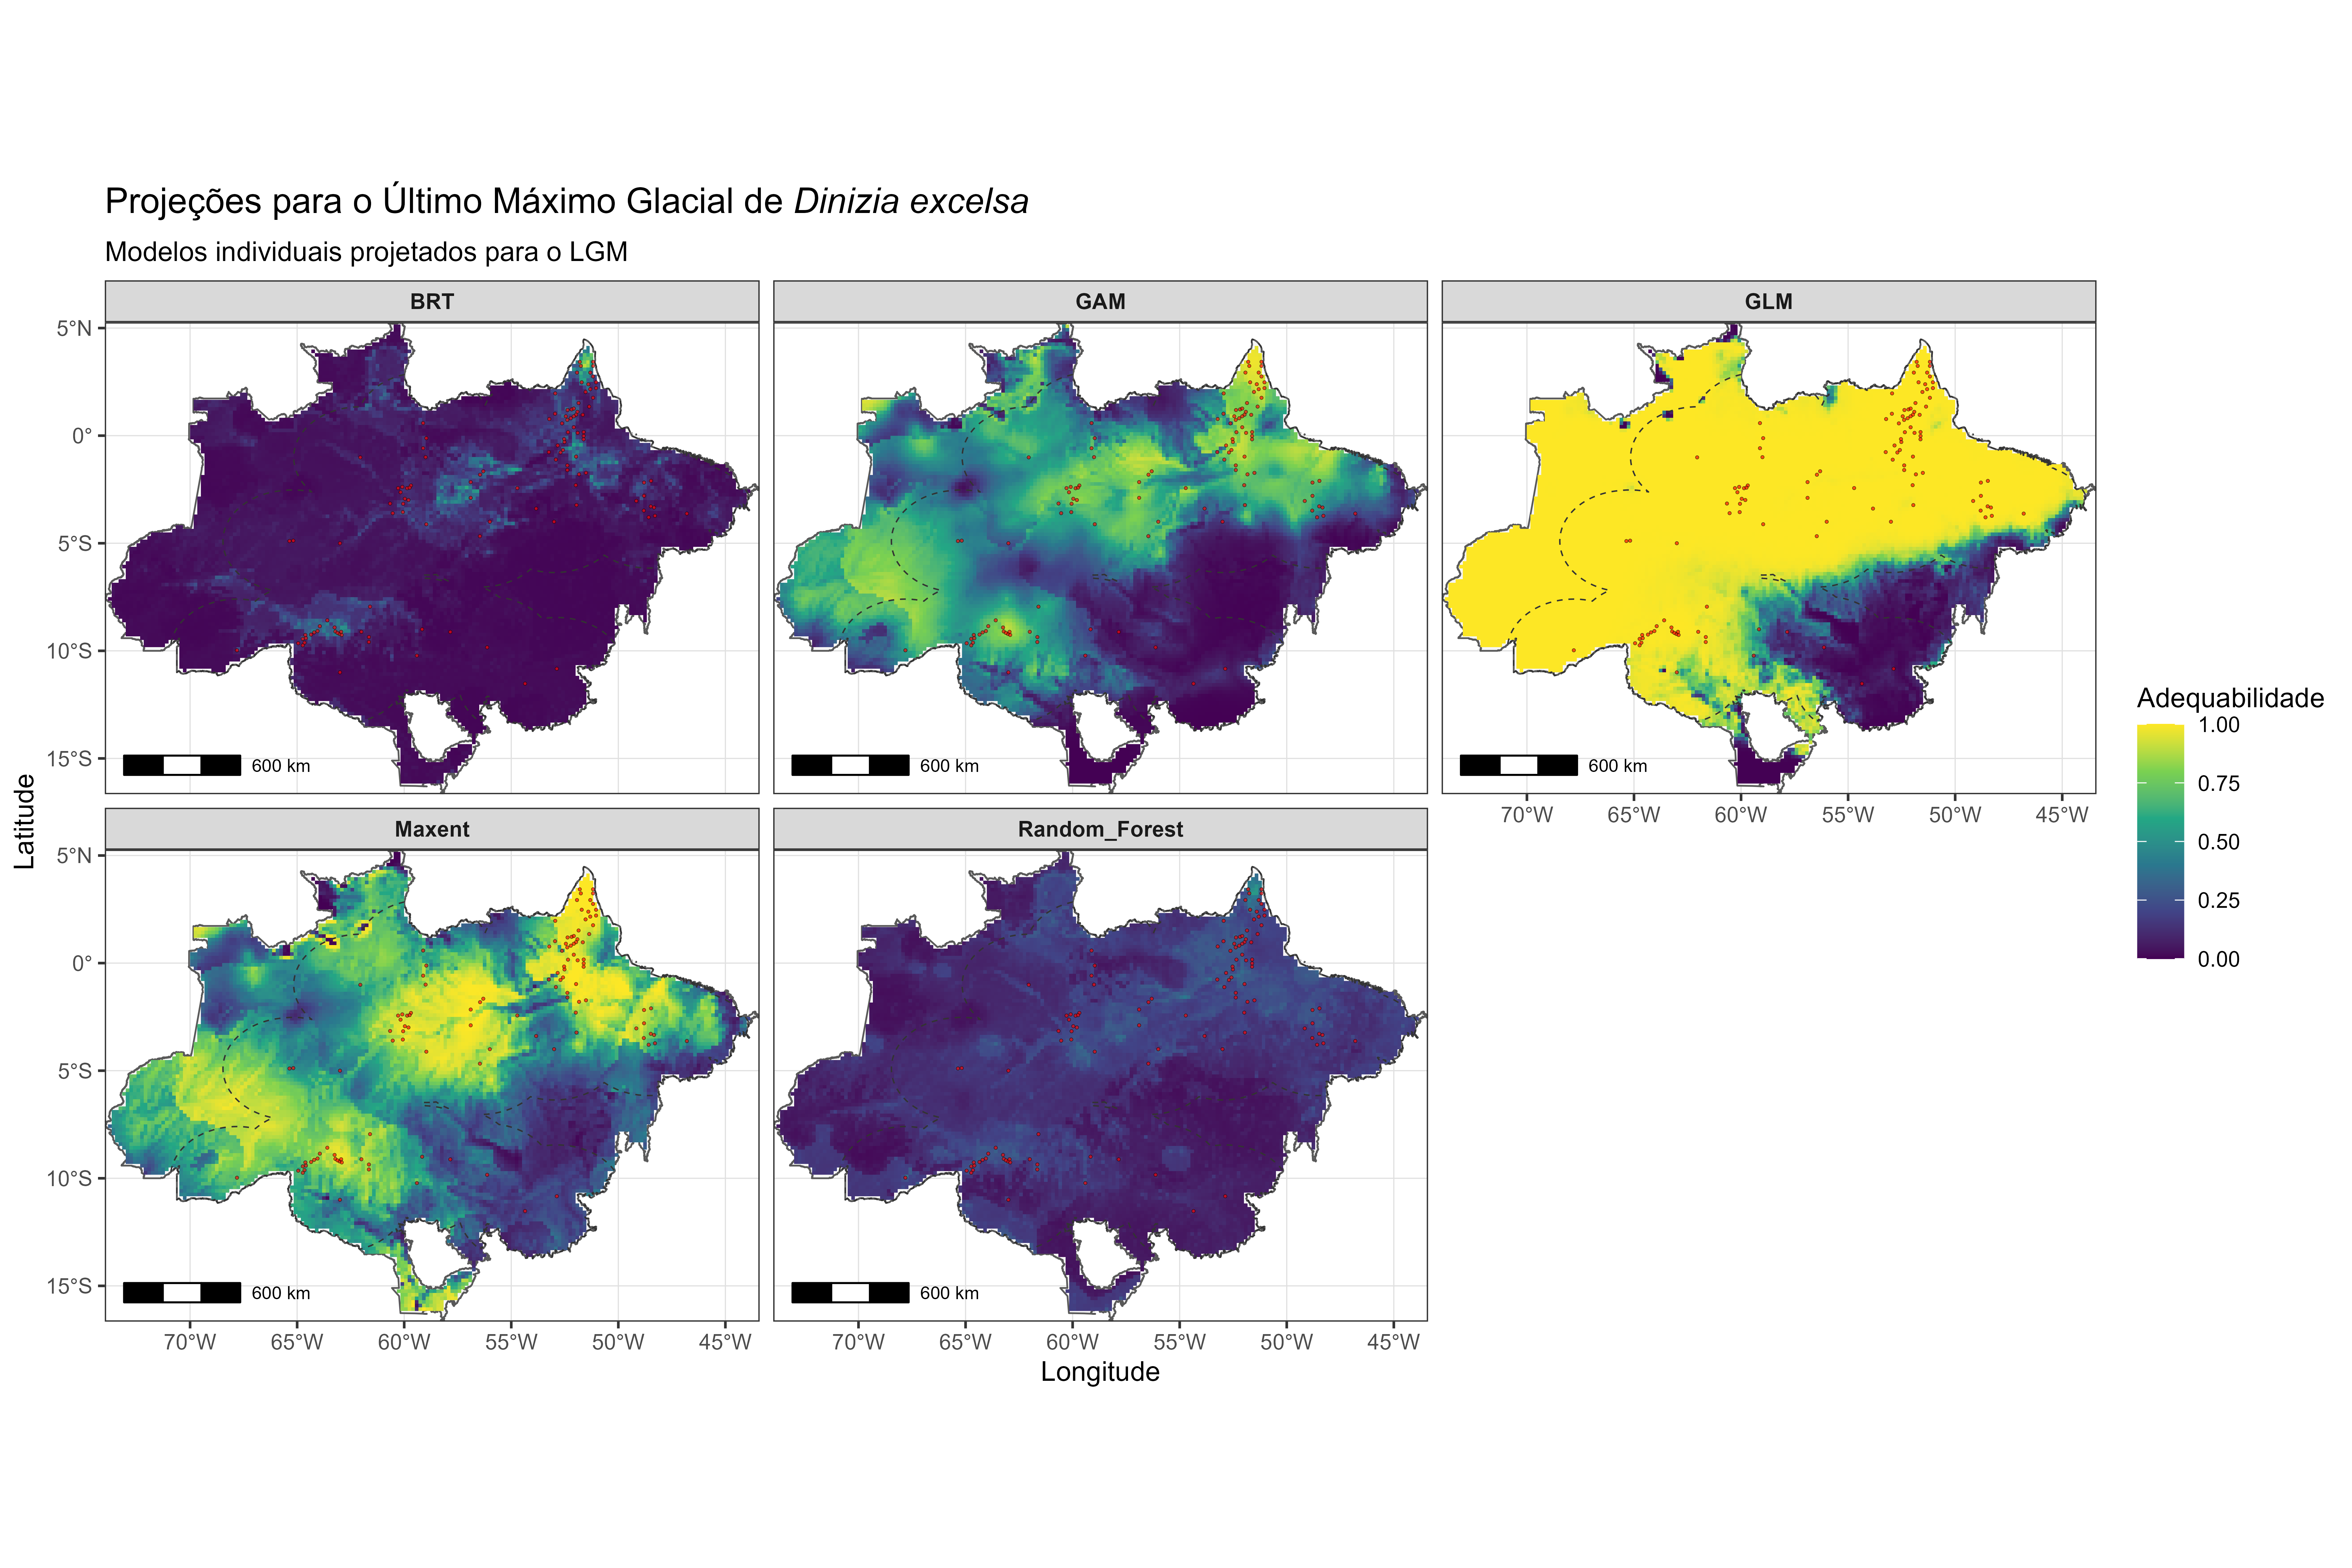
\includegraphics[width=0.98\textwidth]{figuras/unidade15/unidade15_modelos_passado_lgm.png}
	\caption{Projeções dos modelos individuais para \textit{Dinizia excelsa} no Último Máximo Glacial.}
	\label{fig:unidade15_modelos_lgm}
\end{figure}

\section{Ensemble paleoclimático}

As projeções individuais são combinadas em mapas ensemble para cada período paleoclimático.

\rscriptfile{scripts/unidade15/04_ensemble_passado.R}

\begin{figure}[H]
	\centering
	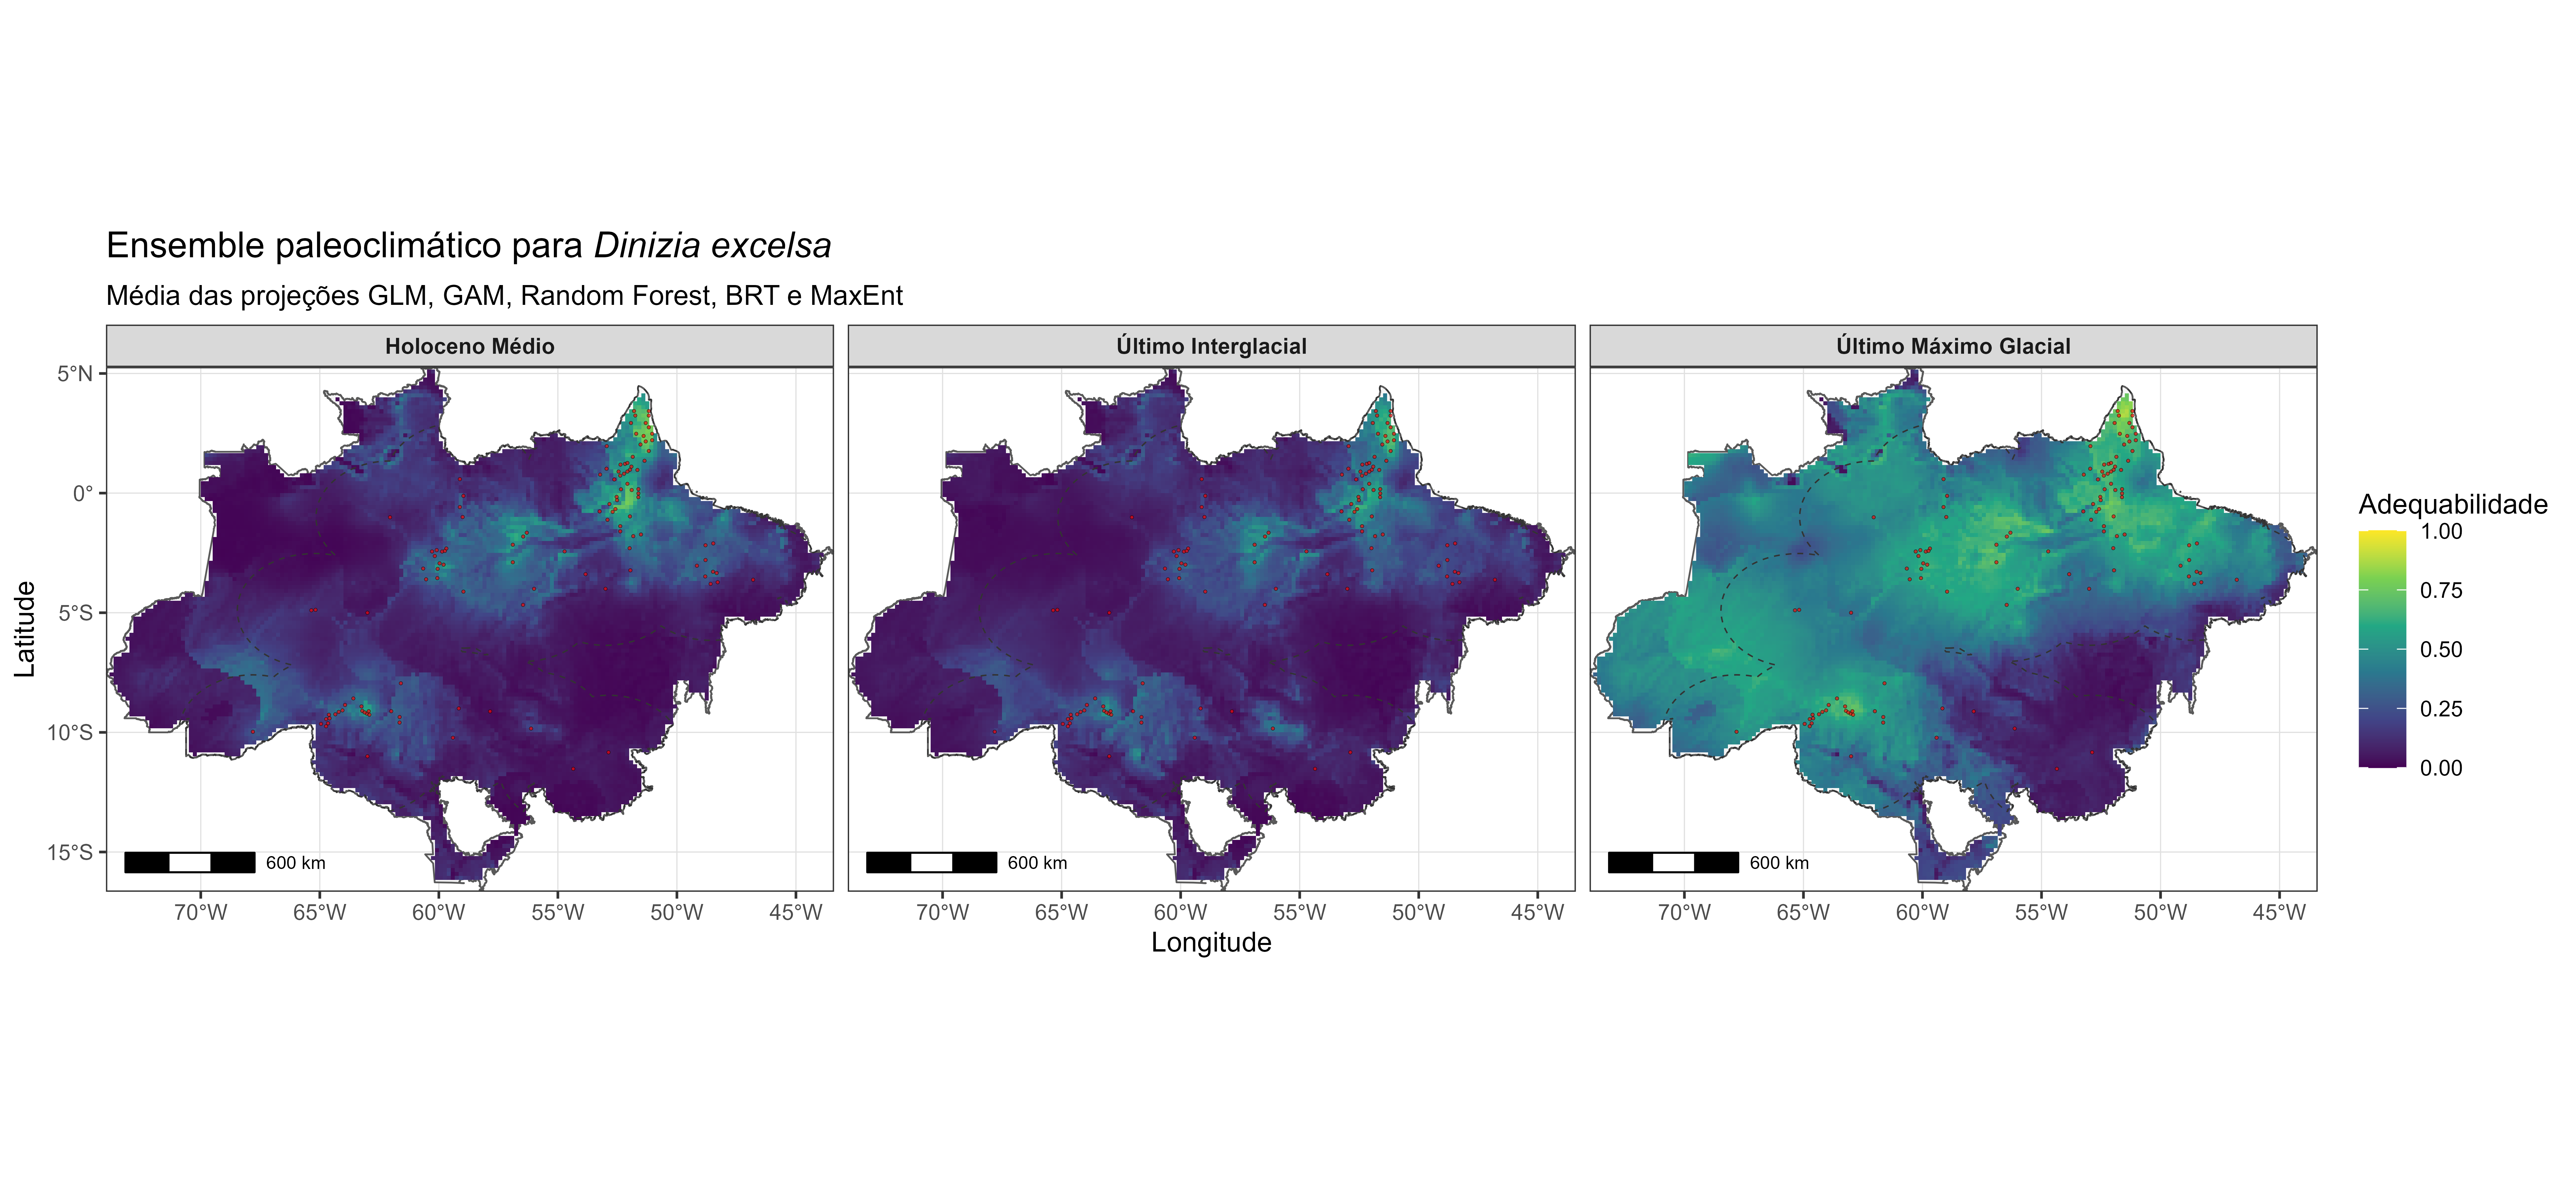
\includegraphics[width=0.96\textwidth]{figuras/unidade15/unidade15_ensemble_passado_periodos.png}
	\caption{Ensemble paleoclimático de adequabilidade ambiental para \textit{Dinizia excelsa}.}
	\label{fig:unidade15_ensemble_passado}
\end{figure}

\section{Trajetória do nicho climático}

A trajetória climática permite comparar o espaço ambiental ocupado no presente com o espaço climático disponível nos períodos passados. Nesta unidade, usamos PCA ambiental para representar mudanças no espaço climático.

\rscriptfile{scripts/unidade15/05_trajetoria_nicho_climatico.R}

\begin{figure}[H]
	\centering
	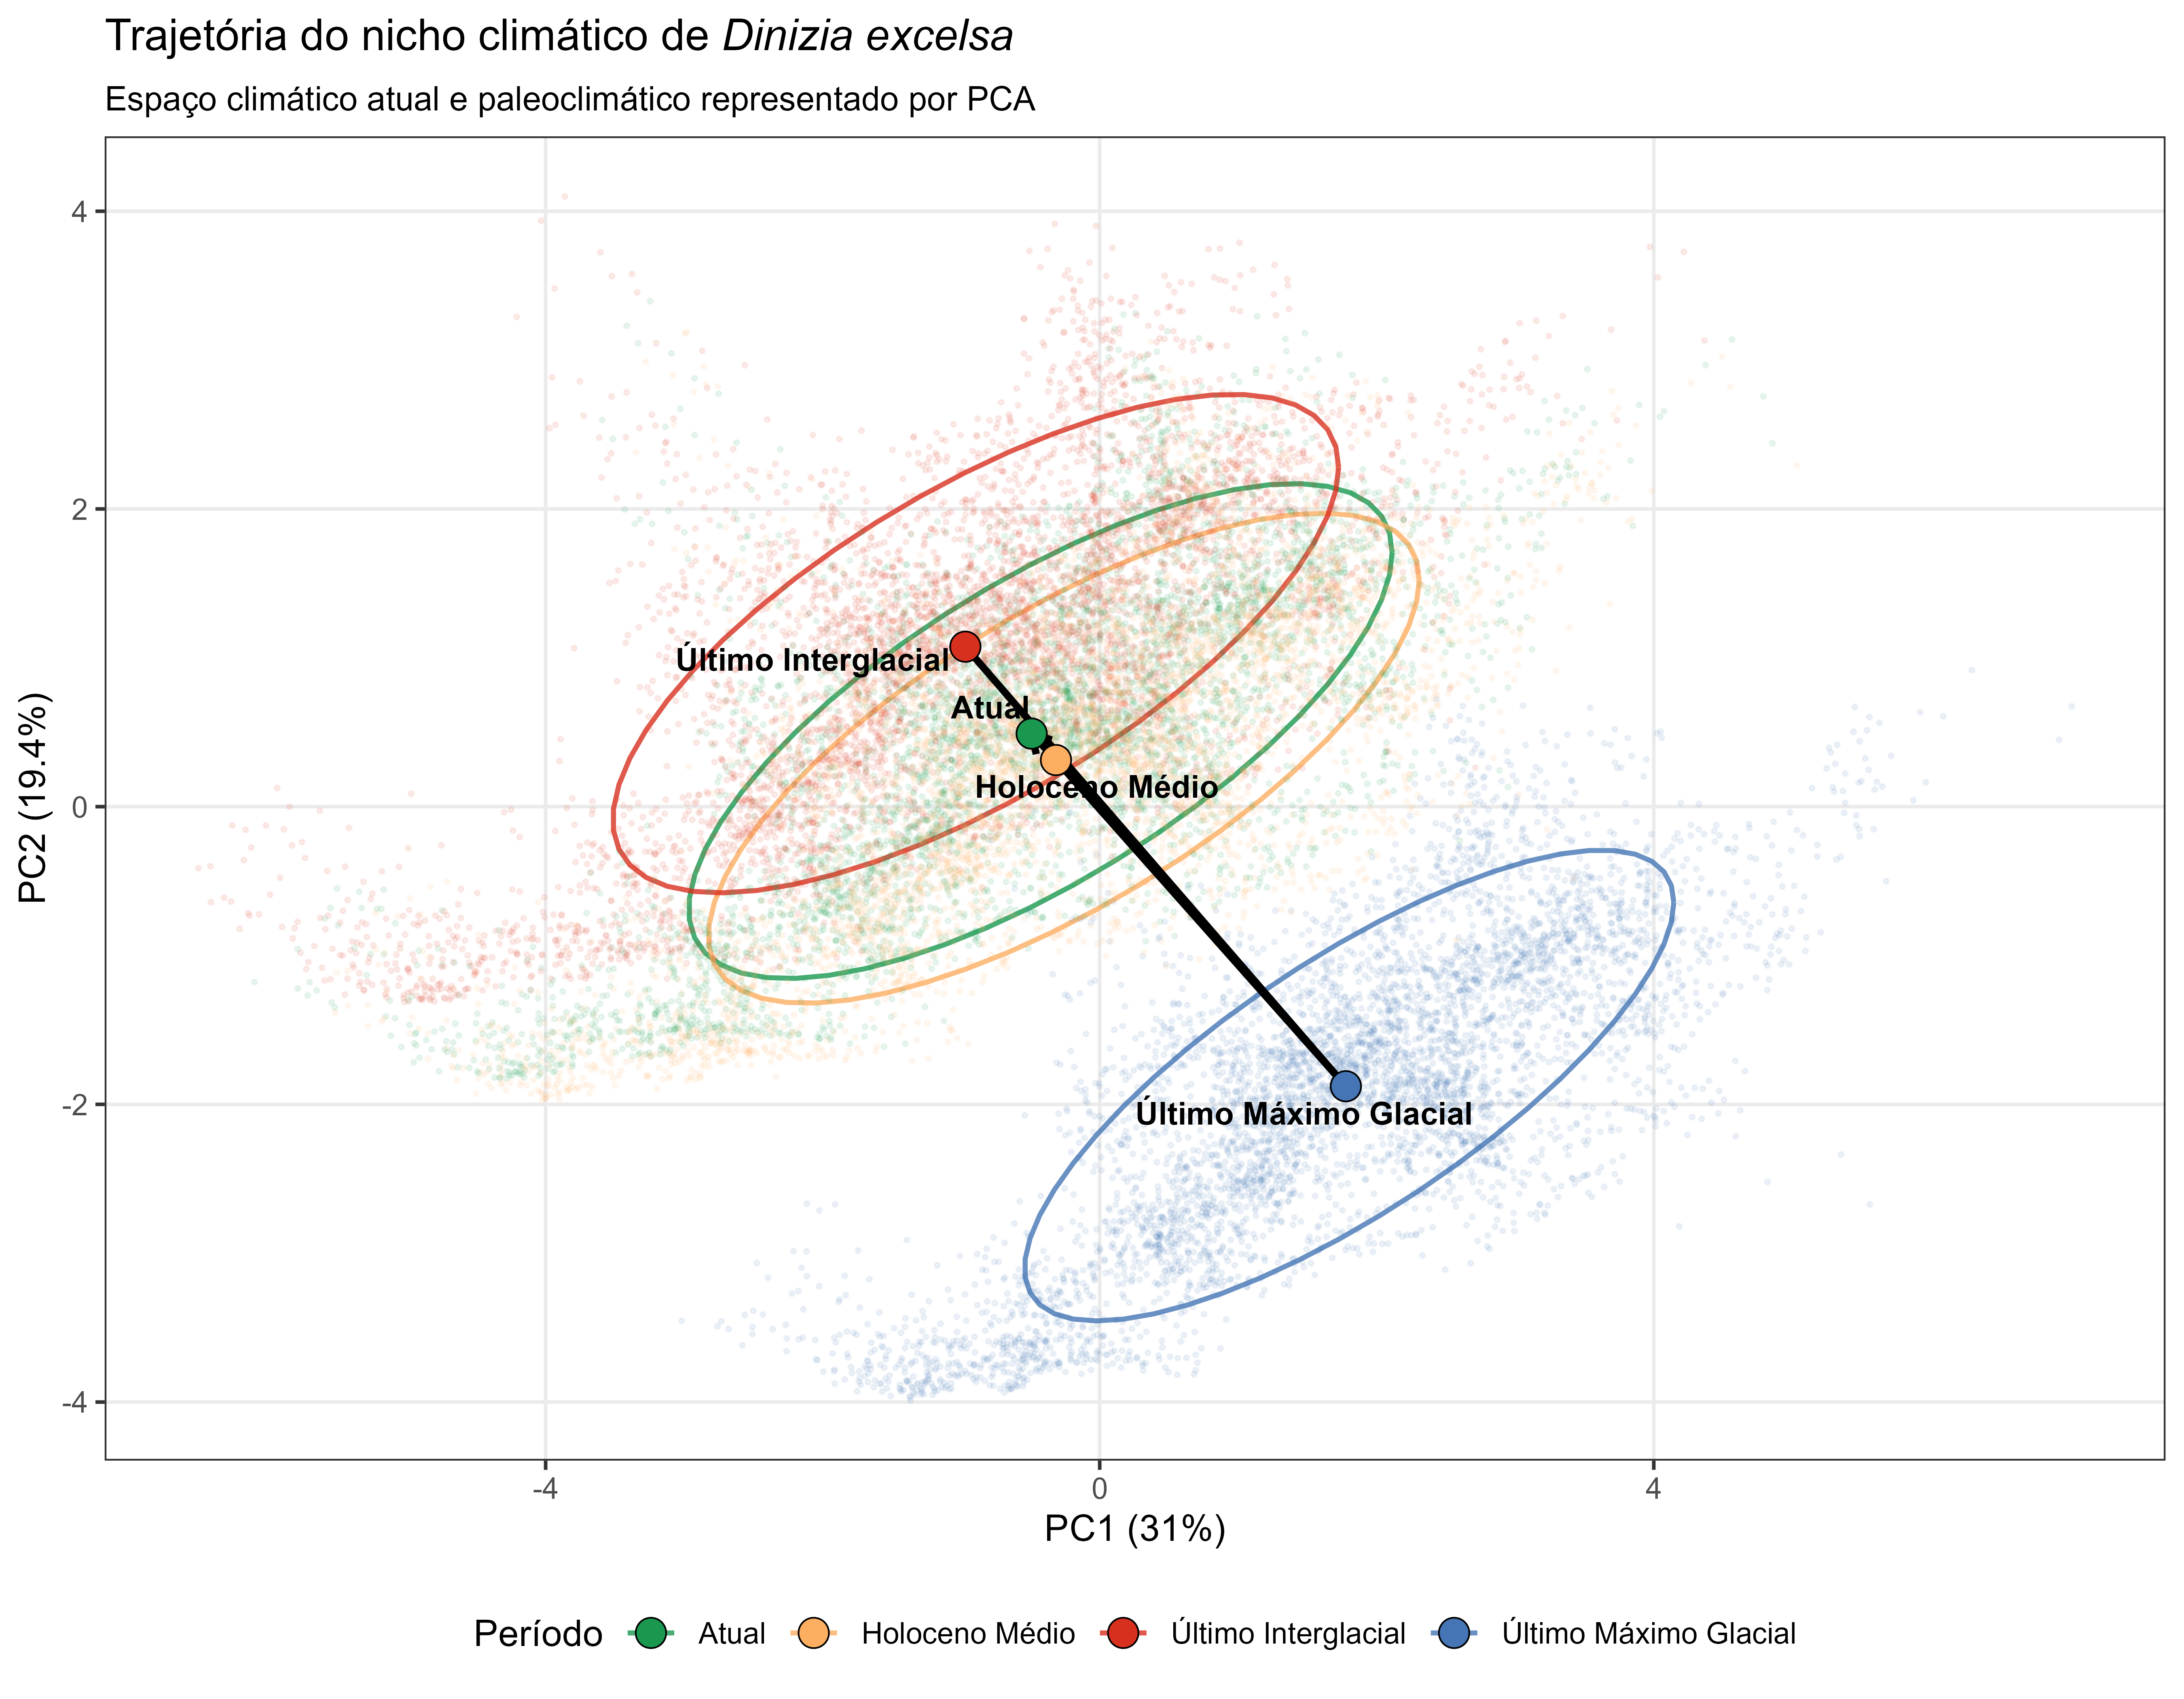
\includegraphics[width=0.88\textwidth]{figuras/unidade15/unidade15_pca_nicho_passado.png}
	\caption{Trajetória do espaço climático atual e paleoclimático para \textit{Dinizia excelsa}.}
	\label{fig:unidade15_pca_nicho_passado}
\end{figure}

\section{Estabilidade histórica e refúgios climáticos}

Áreas climaticamente adequadas no presente e também adequadas em períodos passados podem ser interpretadas como hipóteses de estabilidade climática histórica. Essas áreas não provam refúgios, mas indicam regiões candidatas à persistência de condições favoráveis.

\rscriptfile{scripts/unidade15/06_estabilidade_refugios_paleoclimaticos.R}

\begin{figure}[H]
	\centering
	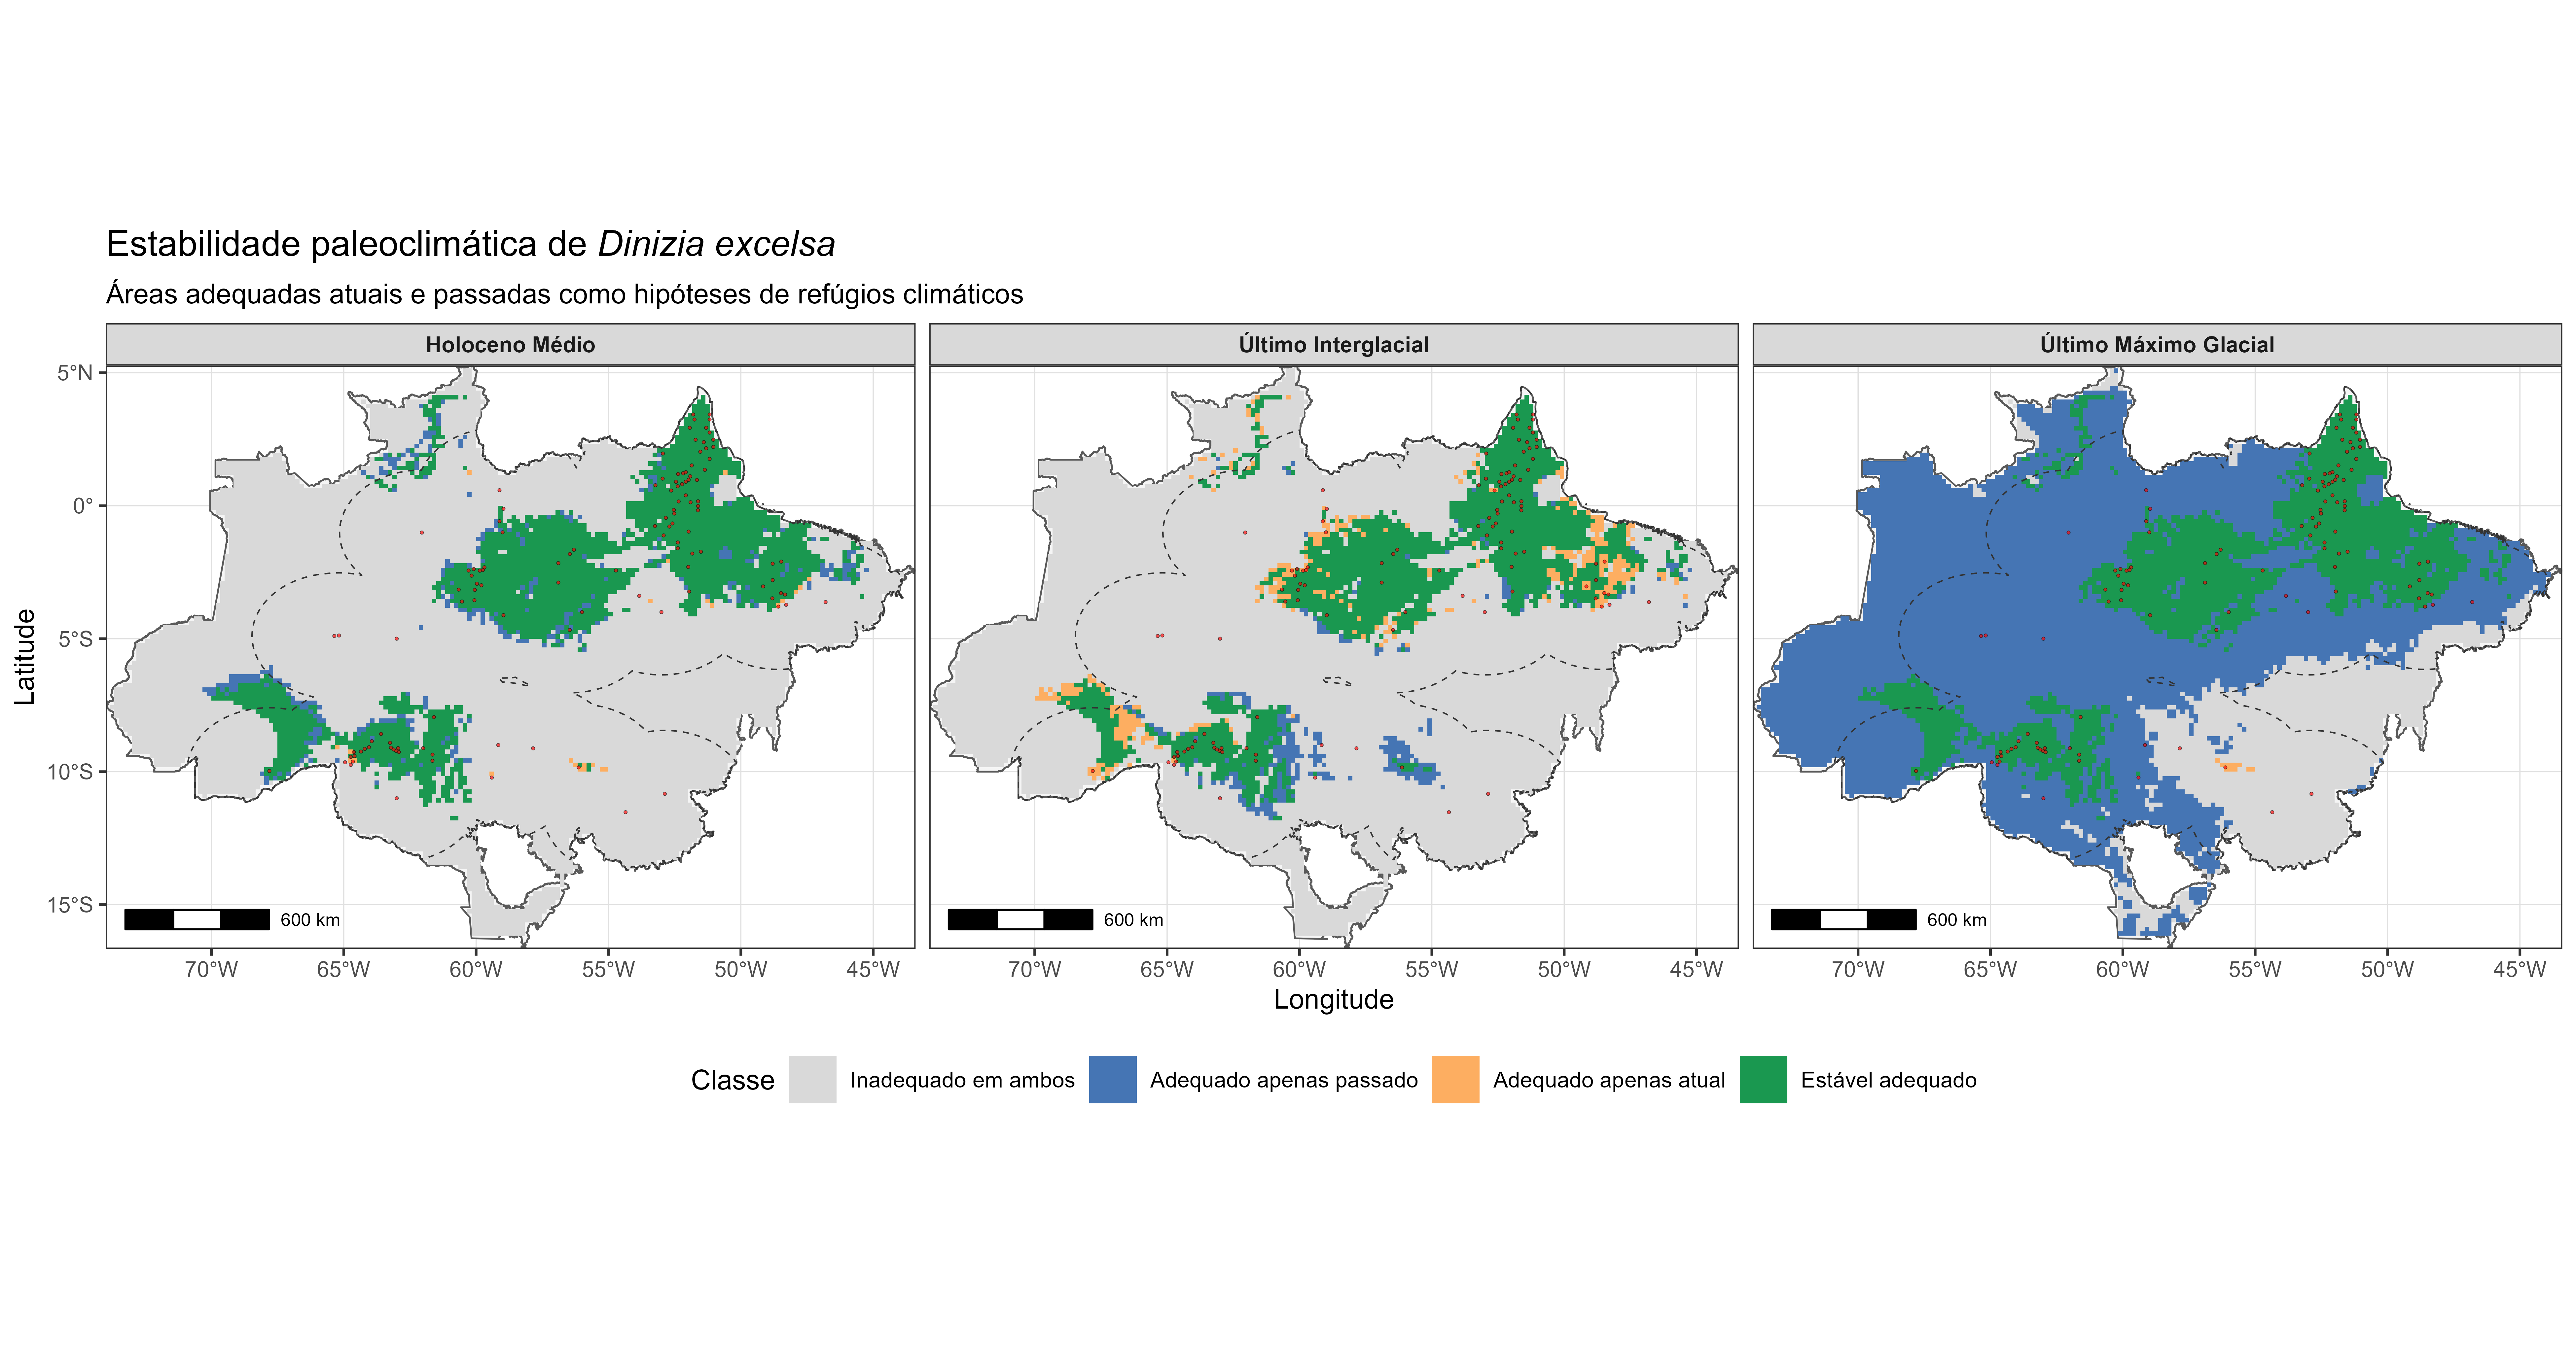
\includegraphics[width=0.96\textwidth]{figuras/unidade15/unidade15_estabilidade_refugios.png}
	\caption{Áreas de estabilidade paleoclimática e possíveis refúgios climáticos para \textit{Dinizia excelsa}.}
	\label{fig:unidade15_refugios}
\end{figure}

\section{Síntese paleoclimática}

\rscriptfile{scripts/unidade15/07_sintese_paleoclimatica.R}

\begin{figure}[H]
	\centering
	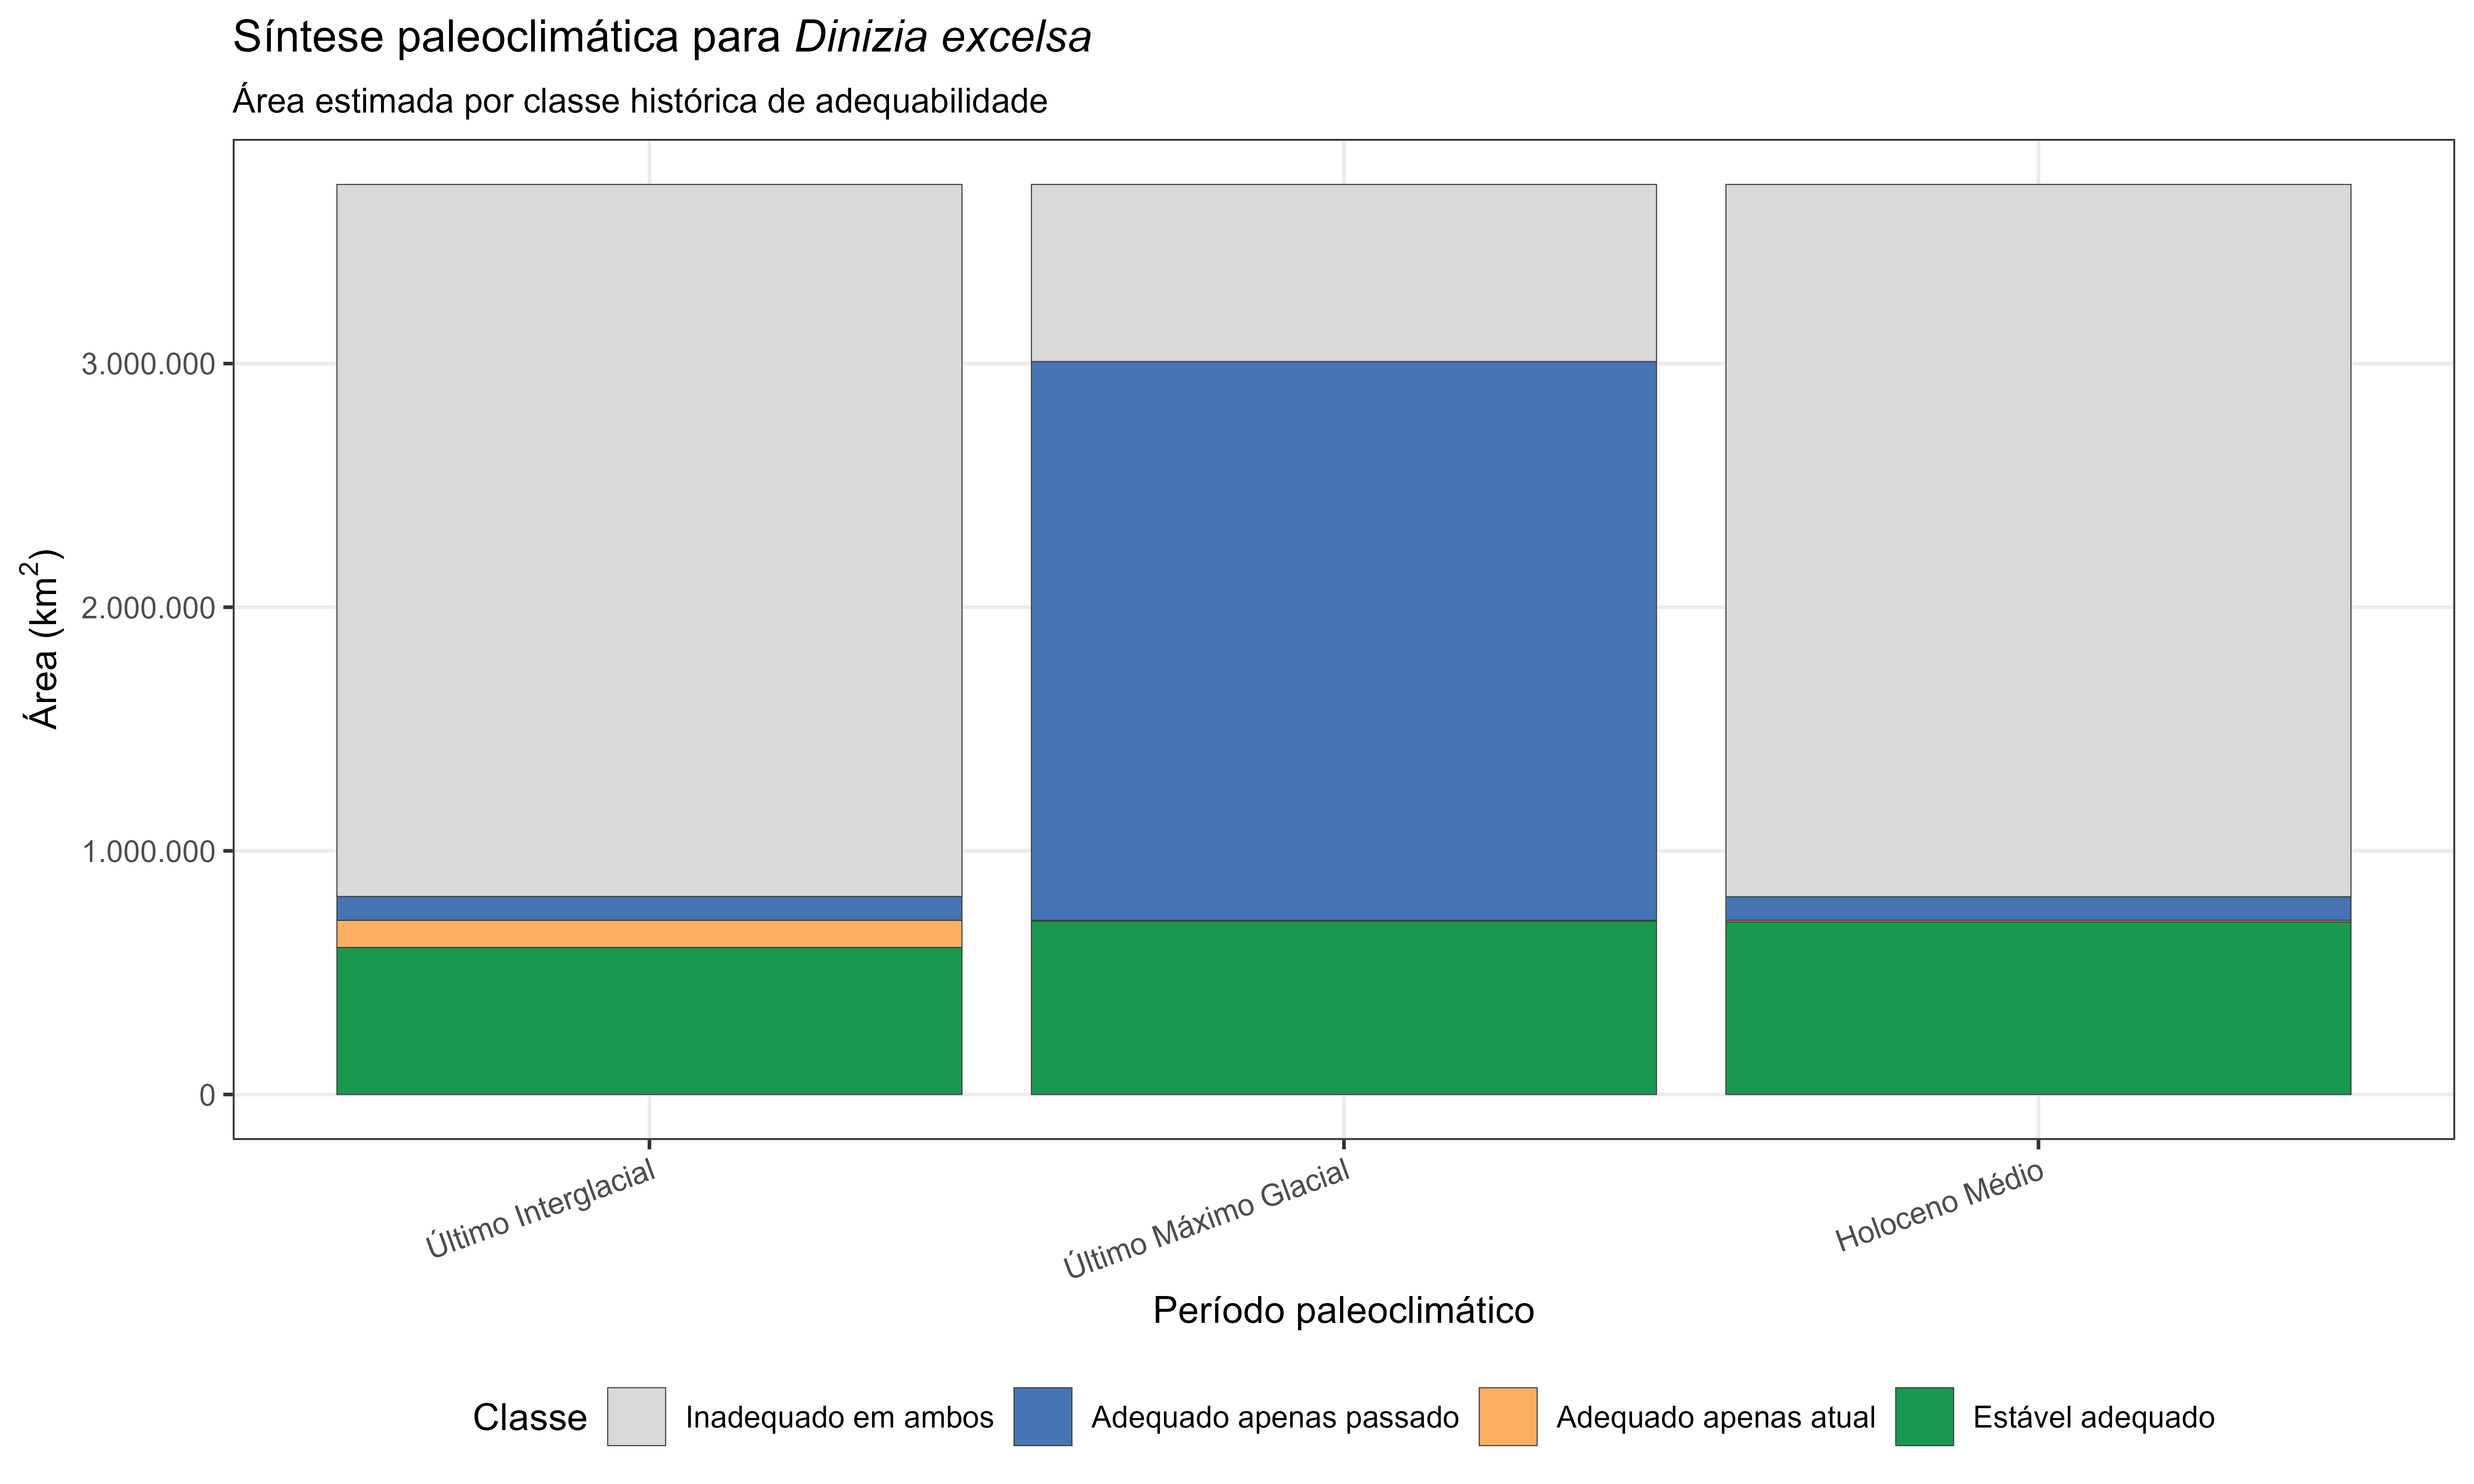
\includegraphics[width=0.88\textwidth]{figuras/unidade15/unidade15_sintese_paleoclimatica.png}
	\caption{Síntese da área adequada estimada para \textit{Dinizia excelsa} em períodos paleoclimáticos.}
	\label{fig:unidade15_sintese}
\end{figure}

\section{Pipeline completo}

\rscriptfile{scripts/unidade15/08_pipeline_paleoclima.R}

\section{Síntese da unidade}

A reconstrução paleoclimática amplia a interpretação dos modelos de distribuição ao conectar o nicho atual da espécie com sua história ambiental. Para \textit{Dinizia excelsa}, esse tipo de análise permite discutir estabilidade climática, possíveis áreas de persistência histórica e hipóteses biogeográficas para a distribuição amazônica contemporânea.

\begin{conceito}[title={\faBook\quad Mensagem central}]
	Projeções paleoclimáticas não mostram onde a espécie ocorreu necessariamente no passado, mas indicam onde o clima passado poderia ter sido compatível com seu nicho climático atual.
\end{conceito}

\section{Exercícios de fixação}

\begin{enumerate}
	\item Explique a diferença entre clima atual, clima futuro e paleoclima em SDM.
	\item O que significa projetar um modelo atual para o Último Máximo Glacial?
	\item Por que áreas estáveis ao longo do tempo podem ser interpretadas como hipóteses de refúgio?
	\item Quais são as principais limitações das projeções paleoclimáticas?
	\item Como a PCA ajuda a interpretar mudanças no espaço climático passado?
	\item Por que conservação de nicho é uma hipótese importante nessa análise?
	\item Como resultados paleoclimáticos podem contribuir para conservação de espécies amazônicas?
\end{enumerate}

% ============================================================
% UNIDADE 16
% ============================================================

